\documentclass[]{article}

\usepackage[italian]{babel}
\usepackage[margin=20mm, footskip = 20pt]{geometry}
\usepackage{array}
\usepackage{tabularx}
\usepackage{graphicx}
\usepackage{subfiles}
\usepackage{hyperref}
\usepackage{nameref}
\usepackage{titlesec}
\usepackage{longtable}
\usepackage[table]{xcolor}
\usepackage{titling}
\usepackage{lastpage}
\usepackage{ifthen}
\usepackage{calc}
\usepackage{soulutf8}
\usepackage{contour}
\usepackage{float}
\usepackage{fancyhdr}
\usepackage{multirow}
\usepackage{pgfgantt}
\usepackage{lscape}

\newcommand{\hr}{\par\vspace{-.1\ht\strutbox}\noindent\hrulefill\par}

\graphicspath{ {./}
	{./commons/res}
}

%--------------------------------------------------
% Comandi per inserire contenuto del documento
%--------------------------------------------------
\makeatletter

\newcommand\appendToGraphicsPath[1]{%
	\g@addto@macro\Ginput@path{{#1}}%
}

\newcommand{\setTitle}[1]{%
	\newcommand{\@phTitle}{#1}%
}
\newcommand{\phTitle}{\@phTitle}

\newcommand{\setDate}[1]{%
	\newcommand{\@phDate}{#1}%
}
\newcommand{\phDate}{\@phDate}

\newcommand{\setUso}[1]{%
	\newcommand{\@uso}{#1}%
}
\newcommand{\uso}{\@uso}

\newcommand{\setVersione}[1]{%
	\newcommand{\@versione}{#1}%
}
\newcommand{\versione}{\@versione}

\newcommand{\disabilitaVersione}{%
	\renewcommand{\setVersione}[1]{}%
	\renewcommand{\versione}{DISABILITATA}
}

\newcommand{\setResponsabile}[1]{%
	\newcommand{\@responsabile}{#1}%
}
\newcommand{\responsabile}{\@responsabile}

\newcommand{\setRedattori}[1]{%
	\newcommand{\@redattori}{#1}%
}
\newcommand{\redattori}{\@redattori}

\newcommand{\setVerificatori}[1]{%
	\newcommand{\@verificatori}{#1}%
}
\newcommand{\verificatori}{\@verificatori}

\newcommand{\setModifiche}[1]{%
	\newcommand{\@modifiche}{#1}%
}
\newcommand{\modifiche}{\@modifiche}

\makeatother 

%--------------------------------------------------
% Comandi per i documenti esterni e il glossario
%--------------------------------------------------

\newcommand{\dext}[1]{\textsc{#1\textsubscript{\textit{D}}}}

\newcommand{\glock}[1]{\textsc{#1\textsubscript{\textit{G}}}}

%--------------------------------------------------
% Comandi per impostare sottotitoli di quarto e quinto livello
%--------------------------------------------------

\setcounter{secnumdepth}{4}
\setcounter{tocdepth}{4}

\titleformat{\paragraph}
{\normalfont\normalsize\bfseries}{\theparagraph}{1em}{}
\titlespacing*{\paragraph}{0pt}{2.25ex plus 1ex minus .2ex}{1.5ex plus .2ex}

\titleformat{\subparagraph}
{\normalfont\normalsize\bfseries}{\thesubparagraph}{1em}{}
\titlespacing*{\subparagraph}{0pt}{1.75ex plus 1ex minus .2ex}{.75ex plus .1ex}

\appendToGraphicsPath{../../../commons/res/}

%------------------------------
%
% COMANDI DI CONFIGURAZIONE
%
%------------------------------

\setTitle{Verbale esterno \#2}

\setVersione{1.0.0}

\setDate{29-12-2020}

\setResponsabile{Valton Tahiraj}

\setRedattori{Lucia Fenu}

\setVerificatori{Paolo Scanferlato}

\setUso{Esterno}

\setModifiche{
	1.0.0 & Valton Tahiraj & Responsabile & 9-01-2020 & Approvazione documento\\
	0.1.0 & Paolo Scanferlato & Verificatore & 06-01-2021 & Verifica Documento\\
	0.0.0 & Lucia Fenu & Redattore & 05-01-2021 & Stesura iniziale}

\begin{document}
	
	% Direttive per la creazione del titolo tramite comando maketitle
\title{\huge \textsc{\phTitle{}} \\
	\vspace{11pt} \large \textsc{\phDate{}}}

\author{} % Non toccare
\date{} % Non toccare

%--------------------
% Frontespizio
%--------------------

% Logo del gruppo
\begin{figure}[t!]
	\centering
	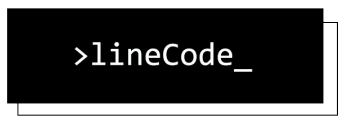
\includegraphics[width=20em]{lclong}
\end{figure}

% Titolo / Nome
\maketitle
\thispagestyle{empty}

% Dati specifici sul doc in forma tabulare
\begin{table}[ht]
	\begin{center}
		\label{tab:Dati sul documento}
		\begin{tabular}{r|l}
			\multicolumn{2}{c}{ \textsc{Dati sul documento} } \\
			\hline
			\textbf{Versione} & \versione{} \\
			\textbf{Uso} & \uso{}  \\
			\textbf{Redattori} & \redattori{} \\
			\textbf{Verificatori} & \verificatori{} \\
			\textbf{Responsabile} & \responsabile{} \\
			\textbf{Destinatari} & lineCode \\
								& prof.\ Vardanega Tullio \\		
								& prof.\ Cardin Riccardo \\
			\ifthenelse{\equal{\uso}{Esterno}}{
								& Sanmarco Informatica
			}{} \\
		\end{tabular}
	\end{center}
\end{table}

\newpage

\renewcommand{\arraystretch}{2} % allarga le righe con dello spazio sotto e sopra
\begin{longtable}[H]{>{\centering\bfseries}m{2cm} >{\centering}m{3.5cm} >{\centering}m{2.5cm} >{\centering}m{3cm} >{\centering\arraybackslash}m{5cm}}
	\rowcolor{lightgray}
	{\textbf{Versione}} & {\textbf{Nominativo}} & {\textbf{Ruolo}} & {\textbf{Data}} & {\textbf{Descrizione}}  \\
	\endfirsthead%
	\rowcolor{lightgray}
	{\textbf{Versione}} & {\textbf{Nominativo}}  & {\textbf{Ruolo}} & {\textbf{Data}} & {\textbf{Descrizione}}  \\
	\endhead%
	\modifiche{}%
\end{longtable}
	
	\newpage
	
	%--------------------------------
	%
	% IL CONTENUTO INIZIA DA QUI
	%
	%--------------------------------
	
	\section{Introduzione}
		\subsection{Luogo e data dell'incontro}
		\begin{itemize}
			\item \textbf{Modalità}: Telematica;
			\item \textbf{Software utilizzato}: Google Meet;
			\item \textbf{Data}: 29 Dicembre 2020;
			\item \textbf{Ora di inizio}: 16:45;
			\item \textbf{Ora di fine}: 17:15.
		\end{itemize}
		
		\subsection{Presenze}
		\begin{itemize}
			\item \textbf{Presenti}: 
			\begin{itemize}
				\item Matteo Alba
				\item Giacomo Bulbarelli
				\item Alessandro Chimetto
				\item Lucia Fenu
				\item Paolo Scanferlato
				\item Valton Tahiraj
			\end{itemize}
			\item \textbf{Assenti}:
			\begin{itemize}
				\item Alessandro Dindinelli
			\end{itemize}
			\item \textbf{Partecipanti esterni}:
			\begin{itemize}
				\item Alex Beggiato (referente, SanMarco Informatica)
			\end{itemize}	
		\end{itemize}
		
		\subsection{Ordine del giorno}
		\begin{enumerate}
			\item Analisi attori;
			\item autenticazione;
			\item ostacoli;
			\item mappa modificabile.
		\end{enumerate}
\newpage	
	\section{Svolgimento}
		\subsection{Analisi attori}
		Alcuni suggerimenti da parte del proponente:
		\begin{itemize}
			\item l'amministratore del sistema, ha la possibilità di aggiungere operatori ed unità e di modificare la mappa;
			\item l'operatore, è l'utente nella quotidianità che usufruisce del sistema;
			\item l'ospite, utente non registrato che accede in sola lettura;
			\item l'unità, invece, fanno parte del sistema ma solo a livello comunicativo coi server; dunque non considerabili come attori;
			\item i pedoni sono un elemento facoltativo e possono essere considerati come attori.
		\end{itemize}
		
	
		\subsection{Autenticazione}
		L'autenticazione per gli utenti ed amministratori è necessaria. \\
		Ogni utente ed ogni entità deve essere registrata.
			
		\subsection{Ostacoli}
		L'unità ha dei sensori e di base se questo trova uno ostacolo deve avere la capacità di fermarsi o di poterlo aggirare. \\
		Il raggio del sensore è importante poiché determina la tempistica su come l'entità deve gestire l'ostacolo.\\
		Oltre al sensore, l'unità comunica costantemente con il sistema sulla sua posizione. \\
		Un ostacolo imprevisto come i pedoni, è facoltativo, in quanto i pedoni lo sono.
		Il pedone può comunicare col sistema sulla loro posizione, ad esempio tramite tecnologia \glock{Bluetooth}.
		
		\subsection{Mappa modificabile}
		La mappa può essere modificata in diversi modi, ad esempio:
		\begin{itemize}
			\item tramite inserimento di un file che dovrà essere validato dal sistema per verificare se la mappa inserita è effettivamente utilizzabile;
			\item tramite interfaccia grafica.
		\end{itemize}
	
	\newpage
	
	\section{Tabella delle decisioni}

\begin{table} [h!]
	\rowcolors{2}{gray!25}{gray!6}
	\begin{center}
		\begin{tabular} { m{2cm} m{14cm} }
			\rowcolor{lightgray}
			\textbf{ID} & \textbf{Decisione}\\
			VE02.1 & Attore: amministratore di sistema, necessario.\\
			VE02.2 & Attore: operatore, necessario. \\
			VE02.3 & Attore: ospite, utente non registrato, necessario. \\
			VE02.4 & Registrazione di ogni unità ed utente. \\
			VE02.5 & Autenticazione degli utenti, necessario. \\
			VE02.6 & L'unità ha dei sensori propri con raggio decisionale. \\
			VE02.7 & L'unità comunica costantemente con il sistema.\\
			VE02.8 & Il pedone può comunicare con il sistema tramite \glock{Bluetooth}.\\
			VE02.9 & La mappa è modificabile tramite inserimento di file da validare.
		\end{tabular}
	\end{center}
\end{table}
\end{document}

